\documentclass{article}
\usepackage{tikz}
\usetikzlibrary{scopes}
\usepackage{verbatim}
\usetikzlibrary{calc,angles,patterns,quotes}


\begin{comment}

:Title: Free body diagrams
:Slug: free-body-diagrams
:Tags: Matrices

Illustration of the classical "bodies connected by a string" problem.
A great advantage of using TikZ for drawing illustrations like this, is that the
drawings can be parameterized. In this example the inclination angle is
parameterized. PGF's mathematical engine is then used to do the necessary calculations.

Note that this example uses the shorthand scope notation in some places.

\end{comment}


\tikzset{
    right angle quadrant/.code={
        \pgfmathsetmacro\quadranta{{1,1,-1,-1}[#1-1]}     % Arrays for selecting quadrant
        \pgfmathsetmacro\quadrantb{{1,-1,-1,1}[#1-1]}},
    right angle quadrant=1, % Make sure it is set, even if not called explicitly
    right angle length/.code={\def\rightanglelength{#1}},   % Length of symbol
    right angle length=1ex, % Make sure it is set...
    right angle symbol/.style n args={3}{
        insert path={
            let \p0 = ($(#1)!(#3)!(#2)$) in     % Intersection
                let \p1 = ($(\p0)!\quadranta*\rightanglelength!(#3)$), % Point on base line
                \p2 = ($(\p0)!\quadrantb*\rightanglelength!(#2)$) in % Point on perpendicular line
                let \p3 = ($(\p1)+(\p2)-(\p0)$) in  % Corner point of symbol
            (\p1) -- (\p3) -- (\p2)
        }
    }
}



\begin{document}

\def\iangle{35} % Angle of the inclined plane
\def\down{-90}
\def\arcr{0.5cm} % Radius of the arc used to indicate angles

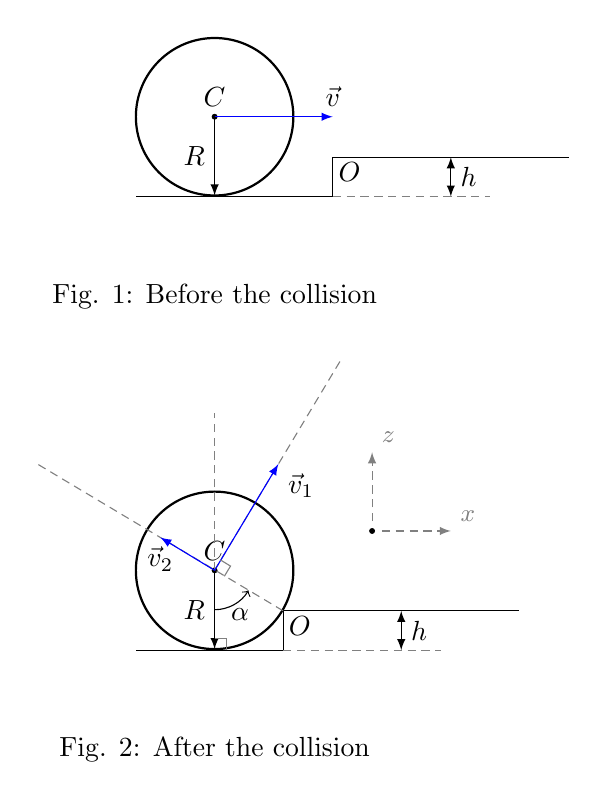
\begin{tikzpicture}[
    force/.style={>=latex,draw=blue,fill=blue},
    axis/.style={densely dashed,gray,font=\small},
    M/.style={rectangle,draw,fill=lightgray,minimum size=0.5cm,thin},
    m/.style={rectangle,draw=black,fill=lightgray,minimum size=0.3cm,thin},
    plane/.style={draw=black,fill=blue!10},
    string/.style={draw=red, thick},
    pulley/.style={thick},
]
\matrix[column sep=1cm, row sep=0.5cm] {
    % initial state
    \node[circle, draw, thick, minimum size=2cm] (ring) {};
    \draw[fill=black] (ring) circle [radius=0.03]; % draw a point in the centre of the ring
    \node[above] at (ring.center) {$C$};

    \draw (ring.south) -- ++(1.5, 0) coordinate (stepbase)
                       -- ++(0, 0.5cm) coordinate (stepcorner)
                       -- node(stepmiddle){} ++(3, 0) node (steprightedge){};

    \draw (ring.south) -- ++(-1cm, 0);
    \node[below right=-0.05cm] at (stepcorner) {$O$};

    % initial velocity vector
    \draw[force, ->] (ring.center) -- ++(1.5cm, 0) node[above]{$\vec{v}$};
    \draw[force, draw=black, ->] (ring.center) -- node[left] {$R$} ++(0, -1cm);

    \draw[force, draw=black, <->] (stepmiddle.center) -- node[right] {$h$} ++(0, -0.5cm) coordinate (stepmiddlebase);
    \draw[axis,-](stepbase) -- (stepmiddlebase) -- ++(0.5, 0);
    \node[below=2cm] at (ring.center) {Fig. 1: Before the collision};

\\
    % just after collision
    \node[circle, draw, thick, minimum size=2cm] (ring) {};
    \draw[fill=black] (ring) circle [radius=0.03]; % draw a point in the centre of the ring
    \node[above] (ring.center) {$C$};

    % draw the floor and the step
    \draw (ring.south) -- ++(0.87cm, 0) coordinate (stepbase)
                       -- ++(0, 0.5cm) coordinate (stepcorner)
                       -- node(stepmiddle){} ++(3, 0) node (steprightedge){};

    \draw (ring.south) -- ++(-1cm, 0);
    \node[below right=-0.05cm] at (stepcorner) {$O$};

    \draw[force, draw=black, ->] (ring.center) -- node[left](rlabel) {$R$} ++(0, -1cm) node (rend) {};

    \draw[force, draw=black, <->] (stepmiddle.center) -- node[right] {$h$} ++(0, -0.5cm) coordinate (stepmiddlebase);
    \draw[axis,-](stepbase) -- (stepmiddlebase) -- ++(0.5, 0);

    \draw[axis,-](stepcorner) -- coordinate(v2end) ([xshift=-2.25cm,yshift=1.35cm]ring.center);
    \draw[axis,-](ring.center) -- coordinate(v1end) ([xshift=1.62cm,yshift=2.7cm]ring.center);

    \draw[axis,-](ring.center) -- ++(0, 2cm);

    \draw[force, ->] (ring.center) -- (v2end) node[below]{$\vec{v}_{2}$};
    \draw[force, ->] (ring.center) -- (v1end) node[below right]{$\vec{v}_{1}$};

    \draw[draw=gray, right angle symbol={v2end}{ring.center}{v1end}];
    \draw[draw=gray, right angle symbol={ring.center}{rend}{stepbase}];
    \pic [draw, ->, "$\alpha$", angle eccentricity=1.3] {angle = rend--ring--stepcorner};


    % draw z-x axes
    \node  at (2, 0.5) (zxorigin){};
    \draw[axis,>=latex,->] (zxorigin) -- ++(1cm, 0) node[above right]{$x$};
    \draw[axis,>=latex,->] (zxorigin) -- ++(0, 1cm) node[above right]{$z$};
    \draw[fill=black] (zxorigin)  circle [radius=0.03]; % draw a point in the centre of the ring

    \node[below=2cm] at (ring.center) {Fig. 2: After the collision};

\\
};
\end{tikzpicture}

\end{document}
